\section{Accelerating the computation of the MUSIC spectrum}
\label{sec:acc-music}

% TODO change the section reference when assembling the reports
% TODO include the new profiling reports
% TODO profile the chain on ARM
% TODO make defines private members in code
The MUSIC spectrum is computed in the \textbf{MUSIC Linear Array} block, whose
functionality was detailed in Report 2, Section 4.4. Through profiling, it was
found that a computationally intensive part is in the vectorial multiplication
used in the denominator of the MUSIC spectrum in formula
\eqref{eq:music-spectrum}.
\begin{equation}
    P_{MUSIC}(\theta) =
        \frac{1}
             {\bm{a}^H(\theta)\bm{V}_N\bm{V}_N^H\bm{a}(\theta)} \\
\label{eq:music-spectrum}
\end{equation}

In the above equation, $\bm{a}(\theta)$ is the basis vector of the signal
subspace, of length M, where M is the size of the antenna array, while
$\bm{V}_N$ is a matrix formed by the eigenvectors of the autocorrelation matrix
$\bm{R}_{xx}$ that are orthogonal to the steering vectors. The product
$\bm{V}_N\bm{V}_N^H$ is therefore a square matrix of size M by M, which we will
further denote as $V_{N_{sq}}$. Its range space is what we call the noise
subspace \cite{cite:ettus-doa}. \\

Both $\bm{a}(\theta)$ and $\bm{V}_{N_{sq}}$ are matrices of complex elements. The
real and imaginary parts of $\bm{a}(\theta)$ are each in the $[-1, 1]$ interval.
As of $\bm{V}_{N_{sq}}$, its range of values is difficult to establish, but in
practice it has been observed that it belongs to the same interval. Therefore,
for the first part of the multiplication, $\bm{a}^H(\theta)\bm{V}_{N_{sq}}$, the
real and imaginary parts of an element of the result cannot exceed the range
$[-M, M]$. This result is a row vector of size 1 by M, which we denote
$X_{1,N}$. \\

We have decided to compute $X_{1,N}$ on the ConnexArray and the final part,
$X_{1,N}\bm{a}(\theta)$, on the ARM processor, due to performance considerations
that will be outlined.

\subsection{Multiplication kernel on the ConnexArray SIMD}
First, we consider the multiplication of row vector of length M by a square matrix
of size M by M, which yields as a result a row vector of length M.
\begin{equation}
    X_{1,N}
    \overset{\Delta}{=}
    \begin{bmatrix}
        a_0   &   a_1   &   \hdots   &   a_{M-1}
    \end{bmatrix}
    \begin{bmatrix}
        v_{0,0}   &   v_{0,1}   &   \hdots   &   v_{0,M-1} \\
        v_{1,0}   &   v_{1,1}   &   \hdots   &   v_{1,M-1} \\
        \vdots    &   \vdots    &   \ddots   &   \vdots    \\
        v_{M-1,0} &   v_{M-1,1} &   \hdots   &   v_{M-1,M-1}
    \end{bmatrix}
\end{equation}
\begin{equation}
    X_{1,N}
    =
    \begin{bmatrix}
        \displaystyle{\sum_{i=0}^{M-1} a_iv_{i,0}} & 
        \displaystyle{\sum_{i=0}^{M-1} a_iv_{i,1}} & 
        \hdots &
        \displaystyle{\sum_{i=0}^{M-1} a_iv_{i,M-1}}
    \end{bmatrix}
    , where
\end{equation}
\begin{equation}
a_i = x_i + jy_i, \quad i = \overline{0, M-1}
\end{equation}
\begin{equation}
v_{i,k} = x_{i,k} + jy_{i,k}, \quad i = \overline{0, M-1}, k = \overline{0, M-1}
\end{equation}

The result can be further written as following:
\begin{equation}
X_{1,N}
=
\begin{bmatrix}
  \displaystyle{\sum_{i=0}^{M-1} (x_ix_{i,0} - y_iy_{i,0}) + 
               j\sum_{i=0}^{M-1} (x_iy_{i,0} + y_ix_{i,0})} \\ 
  \displaystyle{\sum_{i=0}^{M-1} (x_ix_{i,1} - y_iy_{i,1}) + 
               j\sum_{i=0}^{M-1} (x_iy_{i,1} + y_ix_{i,1})} \\
  \hdots \\
  \displaystyle{\sum_{i=0}^{M-1} (x_ix_{i,M-1} - y_iy_{i,M-1}) + 
               j\sum_{i=0}^{M-1} (x_iy_{i,M-1} + y_ix_{i,M-1})} \\ 
\end{bmatrix}^T
\end{equation} \\

The proposed way for computing the result makes use of the arrangement in
Figure \ref{fig:mult-pe} in the ConnexArray processor.
% TODO change the figure with a prettier one
\begin{figure}[H]
    \centering
    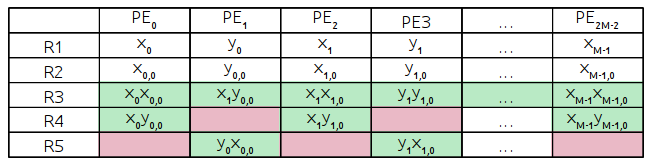
\includegraphics[width=0.75\textwidth]{mult-pe}
    \caption{Arranging the elements in the ConnexArray processing elements}
    \label{fig:mult-pe}
\end{figure}

First, the input array and the input matrix are loaded into the R1 and R2
registers, respectively. The real part of an element will be followed by the
imaginary part of the same element, so for each complex element two PEs are
needed. In the case of the input array, since its elements will have to be
multiplied by each column of the input matrix, they are loaded in blocks of size
M, successively, as shown above. Then, in each PE, we compute the product of the
registers R1 and R2 and store it in R3, thus obtaining the intermediary products
necessary for the real part of the result's elements. \\

To obtain the intermediary products for the imaginary parts, we first shift R2
to the left with one position and store the result in R4. By multiplying R1 with
R4, in half of the PEs (the ones with an even index) we obtain the products in
\eqref{eq:interm-imag-2} and store them in R4.
\begin{equation}
x_iy_{i,k}, \quad i = \overline{0, M-1}, k = \overline{0, M-1}
\label{eq:interm-imag-1}
\end{equation}

Secondly, we shift R2 to the right with one position and store the result in R5.
By multiplying R1 by R5, we obtain the intermediary products in
\eqref{eq:interm-imag-2} in the PEs with an odd index and store them in R5.
\begin{equation}
y_ix_{i,k}, \quad i = \overline{0, M-1}, k = \overline{0,M-1}
\label{eq:interm-imag-2}
\end{equation}

In the figure, the data of interest in the registers is marked by a green
background, and the unnecessary data by a red one.

Next, we move the data in R5 in the PEs with odd index in register R4, so we now
have all the intermediary products for the real and imaginary parts in R3 and
R4, respectively. By performing successive reductions on blocks of size $2M$ on
the aforementioned registers, we obtain the real and imaginary parts of the
elements of $X_{1,N}$. \\

Listing \ref{lst:acc-kernel} contains the kernel that implements the described
algorithm. The kernel is contained in a function that takes as parameters:
\begin{itemize}
  \item \code{process\_at\_once}, a parameter used in case we successively
        multiply more chunks of data
  \item \code{size\_of\_block}, the size of a block on which reduction is performed 
        at once
  \item \code{blocks\_to\_reduce}, on how many blocks the reduction is performed
\end{itemize}

% TODO integrate multiplying part in inline function so that it looks prettier
% explain dependence of data on being mupltiple of 128
\lstset{
    language=C++,
    directivestyle={\color{black}},
    emph={int,char,double,float,unsigned},
    emphstyle={\color{RoyalBlue}}
}
\begin{lstlisting}[
    caption={Kernel for multiplying a row vector with a matrix},
    label={lst:acc-kernel}
]
void multiply_kernel(int process_at_once, int size_of_block, int blocks_to_reduce)
{
  BEGIN_KERNEL("multiply_arr_mat");
    EXECUTE_IN_ALL(
      R25 = 0;
      R26 = 511;
      R30 = 1;
      R31 = 0;
      R28 = size_of_block;  
    )

    EXECUTE_IN_ALL(
      R1 = LS[R25];         // z1 = a1 + j * b1
      R2 = LS[R26];         // z2 = a2 + j * b2
      R29 = INDEX;          // Used later to select PEs for reduction
      R27 = size_of_block;  // Used to select blocks of ARR_SIZE_C for reduction

      R3 = R1 * R2;         // a1 * a2, b1 * b2
      R3 = MULT_HIGH();

      CELL_SHL(R2, R30);    // Bring b2 to the left to calc b2 * a1
      NOP;
      R4 = SHIFT_REG;
      R4 = R1 * R4;         // a1 * b2
      R4 = MULT_HIGH();

      CELL_SHR(R2, R30);
      NOP;
      R5 = SHIFT_REG;
      R5 = R1 * R5;         // b1 * a2
      R5 = MULT_HIGH();

      R9 = INDEX;           // Select only the odd PEs
      R9 = R9 & R30;
      R7 = (R9 == R30);
    )

    EXECUTE_WHERE_EQ(       // Only in the odd PEs
      // Getting -b1 * b2 in each odd cell
      R3 = R31 - R3;        // All partial real parts are in R3

      R4 = R5;              // All partial imaginary parts are now in R4
    )

    REPEAT_X_TIMES(blocks_to_reduce);
      EXECUTE_IN_ALL(
        R7 = (R29 < R27);   // Select only blocks of 8 PEs at a time by
                            // checking that the index is < k * 8
      )
      EXECUTE_WHERE_LT(
        R29 = 129;          // A random number > 128 so these PEs won't be
                            // selected again
        REDUCE(R3);         // Real part
        REDUCE(R4);         // Imaginary part
      )
      EXECUTE_IN_ALL(
        R27 = R27 + R28;    // Go to the next block of 8 PEs
      )
    END_REPEAT;
  END_KERNEL("multiply_arr_mat");
}
\end{lstlisting}

\subsection{Integrating the kernel in a standalone GNURadio out-of-tree module}

In the MUSIC algorithm, the MUSIC spectrum will have a minimum in a point
corresponding to the angle of arrival. An array manifold vector is generated for
a number of \code{d\_spectrum\_length} angles spaced evenly betweem 0 and 180
degrees, which will be used in \eqref{eq:music-spectrum}. Therefore, for each
input signal we will compute \code{d\_spectrum\_length} values of the MUSIC
spectrum. This also means that the matrix $\bm{V}_{N_{sq}}$ will be a factor
in just as many products. \\

In order to assert the functionality of the kernel, we have created a standalone
module named \code{multiply\_cc} that takes as inputs a number of
\code{nr\_arrays} steering vectors of size 1 by \code{arr\_size} and a square
matrix of size \code{mat\_size} and outputs the results of their product, of
size \code{nr\_arrays} by \code{arr\_size}. In reality, we cannot have OOT
(out-of-tree) modules with a variable number of inputs and outputs, so we
linearize the inputs and the outputs.  The input matrix has a column-by-column order,
since this is the way matrices are stored in the libraries Armadillo \cite{cite:armadillo}
and BLAS\cite{cite:blas}. The inputs arrays are row arrays, so they
are considered to be read array-by-array, and the same is also true for the
output. \\

The module uses a \code{forecast} method to ensure that, for an output item,
enough input items are available, according to the corespondence above. The
module is part of a graph that consists of two vector sources, a throttle block,
the \code{multiply\_cc} block and a vector sink. The program that runs the graph
feeds a set of inputs with random values generated in the GNU Octave
\cite{cite:octave} environment and asserts the results by comparing them with the
expected ones computed in Octave. \\

Since the Connex Array has a capacity of \code{vector\_array\_size = 128} PEs,
we will not be able to accomodate inputs with an arbitrarily large number of
elements. The way we proceed is to separate, for each output element that needs
to be produced, the input elements into chunks. How many input arrays can be
multiplied by the same matrix in one job on the ConnexArray depends on the size
of the matrix \code{mat\_size} and is equal to \code{vector\_array\_size /
mat\_size}. A job is considered to be an execution of the kernel on the
ConnexArray. \\

Before each job, the input data has to be \textit{prepared}, meaning that it has
to be scaled and saved into an array of type \code{uint16\_t}. The input matrix
is prepared only once for each output item in the member function
\code{prepareInMatConnex}, while the input arrays have to be prepared for each
chunk using the member function \code{prepareInArrConnex}. \\

After we have the input data in arrays of integers ready, we can launch the
kernel execution. We obtain the output data by reading a number of elements from the
reduction queue. The number of elements read is equal to two times the number of
output items computed in a chunk (because we read a real and an imaginary part). \\

% TODO explain the scaling
Once the data is ready, it has to be scaled back and converted to the
type \code{gr\_complex}, which is an alias for the type
\code{std::complex<float>}, used for the output elements. \\

An important aspect to note is that in this scenario, once the kernel execution
is launched, the program continues executing the instruction in its main thread.
The method that reads the reduction results has to ensure that the ConnexArray
has finished producing the desired number of results and therefore the main
thread will be in a blocking state until that processing is finished. The time
spent waiting for the ConnexArray to finish its execution could be spent doing
other processing in the main thread.

\subsection{Multithreading support for the kernel}

We can take advantage of the time spent with the execution of the kernel by
doing other necessary processing in the main thread. This processing can be
either preparing the elements for the next chunk, preparing the output for the
past chunk or both. Also, with the aid of the kernel we obtain only the
intermediary matrix $\bm{X}_{1xN}$, but the final results needs an additional
multiplication of this result by the steering vector $\bm{a}(\theta)$, and this
could also be computed while waiting for the results on the SIMD processor. \\

Listing \ref{lst:acc-mt-pseudocode} presents a pseudocode that explains the work
flow.
\lstset{
    language=C++,
    directivestyle={\color{black}},
    emph={int,char,double,float,unsigned},
    emphstyle={\color{RoyalBlue}}
}
\begin{lstlisting}[
    caption={Pseudocode explaining the flow of the multithreading program},
    label={lst:acc-mt-pseudocode}
]

prepare_current data();
for all chunks:
  launch_kernel_execution();
  if not last chunk:
    prepare_next_data();
  if not first chunk:
    process_past_data();
  join_threads();
  read_results();
  increment_pointers();
process_past_data();
\end{lstlisting}

The full code for the module that implements the multiplication with
multithreading support cand be found in Listing \ref{lst:acc-mt} in Section
\S\ref{sec:acc-code}. \\

\subsection{Integrating the kernel in the MUSIC DoA chain}

\subsubsection{Adaptations needed for integration}
The kernel that multiplies a row vector with a matrix has to be integrated in
the \textbf{MUSIC Linear Array} block that computes the MUSIC spectrum. Inside
this block, the library Armadillo is necessary to compute the eigenvector
decomposition of the autocorrelation matrix, so it is better to work with data
types specific to Armadillo. An important characteristic of its matrix data
types when considering performance is that they are stored in a column-major
order. This means that elements of a column are contiguous in
memory, so it is desirable to iterate through the columns first and then through
the rows for a faster access to data. \\

The first change, therefore, for integrating the kernel into this block, was to
replace that C++ native vectors of complex elements with the Armadillo
\code{fvec} type and use complex matrices of float elements \code{cx\_fmat}
where possible, which makes for an easier data management. Wherever possible,
the data is passed by references to the functions preparing and processing the
data, to avoid unnecessary copying.


\subsubsection{Results obtained}

The main caveat of using the ConnexArray processor is the conversion from
floating point representation to a fixed point one. This conversion will
inevitably affect precision and it is necessary to assess its effect on the
results. We found that the denomination of the MUSIC spectrum has, on average,
an error of approximately $10^{-4}$, with a maximum error of around $7 \cdot 10^{-4}$.
The problem lies in the fact that, in theory, the value of the denominator is
very close to zero for the angle of arrival and in practice it has a value of
the order of $10^{-5}$ up to $10^{-6}$, which means that the limitations in the
acheivable precision will affect precisely the points of interest. \\

In practice, we found that for a length of the spectrum of 1024 elements, which
translates into an angle resolution of approximately $0,1758^{\circ}$, there are
several points around the angle of interest that are affected by the
insufficient precision. In most cases this means that instead of a clear peak
around a certain angle, there may be two close peaks which will be designated as
the angles of arrival, thus ignoring the correct peak with the lower amplitude
of the MUSIC spectrum. \\

% TODO insert a picture

A solution to this problem would be decreasing the length of the spectrum, but
which will affect the angle resolution. We have found that when decreasing the
length to 512 elements, when the two signal sources are not very close to each
other, we obtain an accuracy of the angles of arrival of $0.1^{\circ}$. For a
length of 256, in the same scenario, the accuracy decreases to $0.5^{\circ}$. \\

We are also interested in how close the two sources can be and the angles of
arrival to still be distinguished. When the container of the MUSIC spectrum has
512 elements, we obtain correct results with a precision of $0.5^{\circ}$ only
when the sources are as close as $20^{\circ}$ to each other. For a length of the
MUSIC spectrum of 256 elements, the sources can be as far as $5^{\circ}$ one from
each other and the accuracy of the results is of around $0.8^{\circ}$. \\

Another solution implies changes in the algorithm that finds the local maximum.
We could introduce a threshold value such as when the algorithm finds two very
close angles (less than one degree apart) it discards one of them and chooses
another that is sufficiently distances from the former. This could eliminate the
"false positives" while not affecting the overall resolution, but with an
additional overhead in finding the local maximum.

\subsubsection{Peformance}
% TODO
